\documentclass[10pt,aspectratio=169]{beamer}
% \documentclass[10pt,aspectratio=169,handout]{beamer}

% silence some Metropolis warnings
\usepackage{silence}
\WarningFilter{beamerthememetropolis}{You need to compile with XeLaTeX or LuaLaTeX}
\WarningFilter{latexfont}{Font shape}
\WarningFilter{latexfont}{Some font}

% define custom colors
\definecolor{dark gray}{HTML}{444444}
\definecolor{light gray}{HTML}{777777}
\definecolor{dark red}{HTML}{BB0000}
\definecolor{dark green}{HTML}{00BB00}

% configure metropolis
\usetheme[numbering=fraction]{metropolis}
\setbeamercolor{background canvas}{bg=white}
\setbeamercolor{frametitle}{bg=dark gray}
\setbeamercolor{alerted text}{fg=dark red}
\setbeamercolor{item projected}{bg=dark red}
\setbeamercolor{local structure}{fg=dark red}
\setbeamersize{text margin left=0.5cm,text margin right=0.5cm}
\setbeamercovered{transparent=10}

% use thicker lines
\makeatletter
\setlength{\metropolis@titleseparator@linewidth}{1pt}
\setlength{\metropolis@progressonsectionpage@linewidth}{1pt}
\makeatother

% custom bullet points
\setbeamertemplate{itemize item}{\color{dark red}$\blacktriangleright$}
\setbeamertemplate{itemize subitem}{\color{dark red}$\blacktriangleright$}
\setbeamertemplate{itemize subsubitem}{\color{dark red}$\blacktriangleright$}
\newcommand{\custombullet}{{\color{dark red}$\blacktriangleright$}\hspace{0.5em}}

% use classic font for math
\usefonttheme[onlymath]{serif}

% imports
\usepackage[english]{babel}
\usepackage[utf8]{inputenc}
\usepackage{amsthm}
\usepackage{amssymb}
\usepackage{amsmath}
\usepackage{amsfonts}
\usepackage{mathtools}
\usepackage{mathabx}
\usepackage{stmaryrd}
\usepackage{graphicx}
\usepackage{hyperref}
\usepackage{xfrac}
\usepackage{appendixnumberbeamer}

% check and x marks
\usepackage{pifont}
\newcommand{\cmark}{{\color{dark green}\ding{51}}\hspace{0.3em}}
\newcommand{\xmark}{{\color{dark red}\ding{55}}\hspace{0.5em}}

% diagrams
\usepackage{tikz}
\usetikzlibrary{decorations.pathreplacing}

% references
\usepackage[natbibapa]{apacite}
\bibliographystyle{apacite}
\renewcommand{\bibsection}{}

% use ampersands instead of "and" for text citations
\AtBeginDocument{\renewcommand{\BBAB}{\&}}

% possessive cites
\makeatletter
\patchcmd{\NAT@test}{\else \NAT@nm}{\else \NAT@nmfmt{\NAT@nm}}{}{}
\DeclareRobustCommand\citepos
  {\begingroup
   \let\NAT@nmfmt\NAT@posfmt
   \NAT@swafalse\let\NAT@ctype\z@\NAT@partrue
   \@ifstar{\NAT@fulltrue\NAT@citetp}{\NAT@fullfalse\NAT@citetp}}
\let\NAT@orig@nmfmt\NAT@nmfmt
\def\NAT@posfmt#1{\NAT@orig@nmfmt{#1's}}
\makeatother

% spaced-out lists
\newenvironment{wideitemize}{\itemize\addtolength{\itemsep}{10pt}}{\enditemize}
\newenvironment{wideenumerate}{\enumerate\addtolength{\itemsep}{10pt}}{\endenumerate}

% replace footnotes with buttons
\usepackage[absolute,overlay]{textpos}
\newcounter{beamerpausessave}
\newcommand{\always}[1]{
    \setcounter{beamerpausessave}{\value{beamerpauses}}
    \setcounter{beamerpauses}{0}
    \pause
    #1 
    \setcounter{beamerpauses}{\value{beamerpausessave}}
    \addtocounter{beamerpauses}{-1}
    \pause
}
\newcommand{\buttons}[1]{\always{
    \begin{textblock*}{\paperwidth}(0.015\textwidth, 1.022\textheight)
        \scriptsize
        #1
    \end{textblock*}
}}
\newcommand{\appendixbuttons}[1]{\always{
    \begin{textblock*}{\paperwidth}(0.015\textwidth, 1.043\textheight)
        \scriptsize
        #1
    \end{textblock*}
}}
\newcommand{\goto}[2]{\hyperlink{#1}{{\color{dark red}$\smalltriangleright$} #2}\hspace{0.5em}}
\newcommand{\goback}[2]{\hyperlink{#1}{{\color{dark red}$\smalltriangleleft$} #2}\hspace{0.5em}}

% custom appendix
\renewcommand{\appendixname}{\texorpdfstring{\translate{Appendix}}{Appendix}}

% change color of cites and URLs
\let\oldcite\cite
\let\oldcitet\citet
\let\oldcitep\citep
\let\oldcitepos\citepos
\let\oldcitetalias\citetalias
\let\oldcitepalias\citepalias
\let\oldurl\url
\def\cite#1#{\citeaux{#1}}
\def\citet#1#{\citetaux{#1}}
\def\citep#1#{\citepaux{#1}}
\def\citepos#1#{\citeposaux{#1}}
\def\citetalias#1#{\citetaliasaux{#1}}
\def\citepalias#1#{\citepaliasaux{#1}}
\def\url#1#{\urlaux{#1}}
\newcommand*\citeaux[2]{{\color{light gray}\oldcite#1{#2}}}
\newcommand*\citetaux[2]{{\color{light gray}\oldcitet#1{#2}}}
\newcommand*\citepaux[2]{{\color{light gray}\oldcitep#1{#2}}}
\newcommand*\urlaux[2]{{\color{light gray}\oldurl#1{#2}}}
\newcommand*\citeposaux[2]{{\color{light gray}\oldcitepos#1{#2}}}
\newcommand*\citetaliasaux[2]{{\color{light gray}\oldcitetalias#1{#2}}}
\newcommand*\citepaliasaux[2]{{\color{light gray}\oldcitepalias#1{#2}}}

% custom math commands
\DeclareMathOperator*{\argmax}{argmax}
\DeclareMathOperator*{\argmin}{argmin}
\renewcommand{\Pr}{\mathbb{P}}
\newcommand{\E}{\mathbb{E}}
\newcommand{\Var}{\mathbb{V}}
\newcommand{\Cov}{\mathbb{C}}
\newcommand{\overbar}[1]{\mkern 1.5mu\overline{\mkern-1.5mu#1\mkern-1.5mu}\mkern 1.5mu}

% tables
\usepackage{booktabs}
\usepackage{colortbl}
\usepackage{multirow}
\usepackage{makecell}
\arrayrulecolor{dark red}

% custom date
\usepackage{datetime}
\newdateformat{monthyeardate}{\monthname[\THEMONTH] \THEYEAR}

% fix pauses with graphics
\usepackage{fixpauseincludegraphics}


\usepackage{tabularx}
\usepackage{dcolumn}
\usepackage{ragged2e}
\usepackage{multirow,multicol,dcolumn}




\begin{document}
\title{Conduct}
\author{Chris Conlon}
\institute{Grad IO}
\date{\today}

\frame{\titlepage}


\begin{frame}[plain]{Conduct Testing in Industrial Organization}
Foundational Empirical IO Question: How do we observe data on price and quantity and infer which model of firm behavior generated those outcomes?

\begin{itemize}
\item Early work: Porter (1983), Bresnahan (1982,1987)
\item Subsequent work defined the ``menu" approach: Nevo (1998, 2001), Villas-Boas (2007) 
\item Recent revival of ``internalization'' parameters: Miller and Weinberg (2017), Crawford, Lee, Whinston, and Yurukoglu (2017), Pakes (2017)
\item Parallel work by: Duarte, Magnolfi, Sølvsten, Sullivan (2022) which test is best (RV). Magnolfi, Quint, Sullivan, Waldfogel (2022) Should we test or estimate?
\item Applications of our test: Starc and Wollman (2022), Scuderi (2022), others?
\end{itemize}
Is conduct testable? Berry and Haile (2014): yes.
\end{frame}


\begin{frame}{Conduct Testing in Industrial Organization}
\begin{itemize}
\item Absent additional restrictions, we cannot generally look at data on $(P,Q)$ and decide whether or not collusion is taking place.
\begin{itemize}
\item You say we started colluding at date $t$, I say we received a correlated shock to $mc$.
\end{itemize}
\item We can make progress in two ways: (1) parametric restrictions on marginal costs; (2) exclusion restrictions on supply.
\begin{itemize}
\item Most of the literature focuses on (1) by assuming something like: $\ln mc_{jt} = x_{jt} \gamma_1 + w_{jt} \gamma_2 + \omega_{jt}$.
\item In principle (2) is possible if we have instruments that shift demand for products but not supply. (These are much easier to come up with than ``supply shifters''). (This is the point Berry Haile 2014 make).
\end{itemize}
\end{itemize}
\end{frame}



\begin{frame}{A famous plot (Bresnahan 87)}
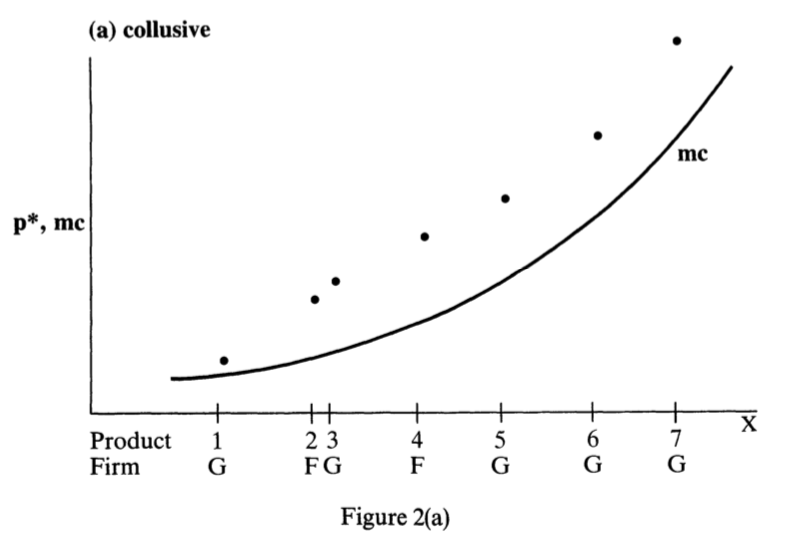
\includegraphics[width = 6.6cm]{./resources/bres_plot1.png}
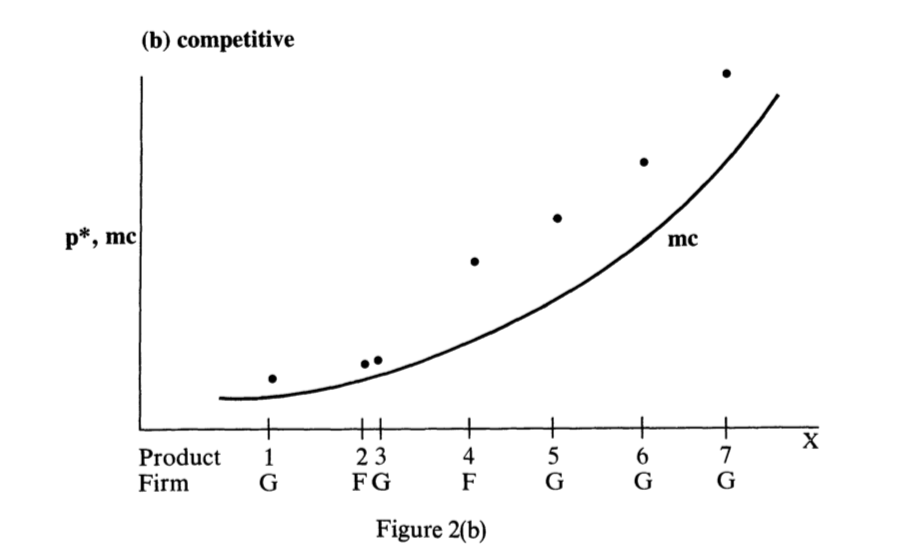
\includegraphics[width = 6.9cm]{./resources/bres_plot2.png}\\
Bresnahan (1980/1982) recognized this problem: we need ``rotations of demand''.
\end{frame}


\begin{frame}[plain]{Conduct Testing in Pictures (Berry Haile 2014)}
\begin{center}
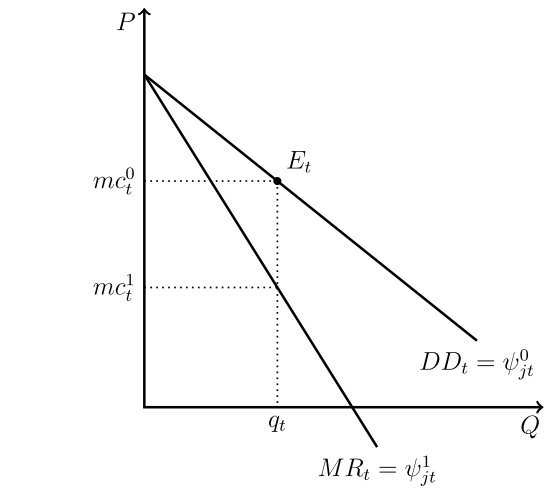
\includegraphics[width = 6.5cm]{resources/berryhaile1.png}
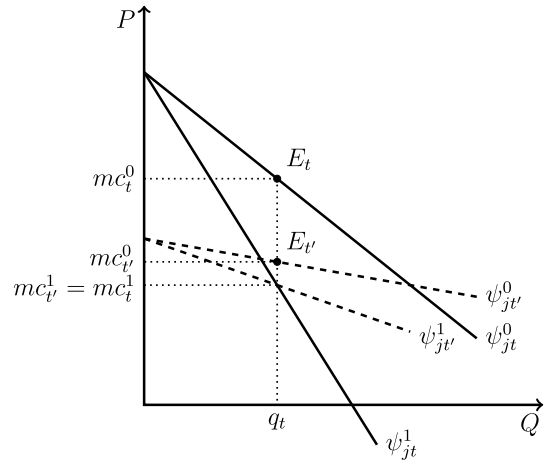
\includegraphics[width = 6.5cm]{resources/berryhaile2.png}
\end{center}
\small{Figure 2(ab) from Berry and Haile (2014), Example 1.}
\end{frame}




\begin{frame}{Setup: Notation and Utility}
We begin with a relatively standard BLP-style differentiated products setup.\\

\begin{itemize}
    \item Markets $t$
    \item Products $j$
    \item Data $\chi_t = \{(\textrm{x}_{jt},\textrm{v}_{jt},\textrm{w}_{jt})$ for all $j \in \mathcal{J}_t\}$.
    \item Market Shares $\mathcal{S}_t = [s_{1t}, \ldots, s_{Jt}, s_{0t}]$.
    \item Prices $\mathbf{p}_t = [p_{1t}, \ldots, p_{Jt}]$.
    \item Consumers $i$ with demographics $y_{it}$ (income, presence of kids)
\end{itemize}
\end{frame}

\begin{frame}
\frametitle{Testing Conduct: Multiproduct Bertrand Example}
\small
We generalize the $\mathcal{H}(\kappa)$ and derive multi-product Bertrand FOCs:
\begin{align*}
\arg \max_{p \in \mathcal{J}_f} \pi_f (\mathbf{p}) &= \sum_{j \in \mathcal{J}_f} (p_j - c_j) \cdot q_j(\mathbf{p}) +  \alert{\kappa_{fg} \sum_{j \in \mathcal{J}_g} (p_j - c_j) \cdot q_j(\mathbf{p})} \\
\rightarrow 0&= q_j(\mathbf{p}) + \sum_{k \in (\mathcal{J}_f,\mathcal{J}_g)} \alert{\kappa_{fg}}\cdot (p_k - c_k) \frac{\partial q_{k}}{\partial p_j}(\mathbf{p}) 
\end{align*}
\begin{itemize}
\item Instead of $0$'s and $1$'s we now have $\kappa_{fg} \in [0,1]$ representing how much firm $f$ cares about the profits of $g$.
\begin{itemize}
\item If $f$ and $g$ merge (or fully coordinated) then $\kappa_{fg} =1$
\item Often in the real world firms cannot reach fully collusive profits and $\kappa_{fg} \in (0,1)$.
\item Evidence that $\kappa_{fg} > 0$ is not necessarily evidence of malfeasance, just a deviation from \alert{static Bertrand pricing} (e.g. Cournot, Dynamics, etc.)
\end{itemize}
\end{itemize}
\end{frame}


\begin{frame}{Testing Conduct: Multiproduct Bertrand Example}
\begin{itemize}
\item Recall the $\Delta$ matrix which we can write as $\Delta=\tilde{\Delta}\, \odot \mathcal{H}(\kappa)$, where $\odot$ is the element-wise or Hadamard product of two matrices. 
\begin{itemize}
\item $\tilde{\Delta}$ is the matrix of demand derivatives with $\Delta{(j,k)} = \frac{\partial q_j}{\partial p_k}$ for all elements.
\item $\mathcal{H}(\kappa)=\kappa_{fg}$ for products owned by $(f,g)$ where $\kappa_{ff}=1$ always.
\end{itemize}
\item Mergers are about changing $0$'s to $1$'s in the $\mathcal{H}(\kappa)$ matrix.
\item Matrix form of FOC: $q(\mathbf{p}) = \Delta(\mathbf{p},\kappa)\cdot(\mathbf{p}-\mathbf{mc})$
\item $\mathbf{mc} =  \mathbf{p} - \underbrace{\Delta(\mathbf{p}, \theta_2, \kappa)^{-1} s(\mathbf{p})}_{\eta(\mathbf{p},\mathbf{s},\theta_2,\kappa)}$
where $\eta_{jt}$ is the markup.
\end{itemize}
\end{frame}

\begin{frame}
\frametitle{Reasons for Deviations from Multiproduct Bertrand}
\small
\begin{description}
\item[Biased estimates of own and cross price derivatives:] For anything to work, you have correct estimates of $\tilde{\Delta}$. My prior is most papers \alert{underestimate} diversion ratios for close substitutes.
\item[Vertical Relationships:] Who sets supermarket prices? Just the retailer? Just the manufacturer? Some combination of both? Retailers tend to \alert{soften} downstream price competition.
\item[Faulty Timing Assumptions:] Bertrand is a simultaneous move pricing game. Lots of alternatives (Stackelberg leader-follower, Edgeworth cycles, etc.).
\item[Dynamics and Dynamic Pricing:] Forward looking firms or consumers might not set static Nash prices. [e.g. Temporary Sales, Switching Costs, Network Effects, etc.]
\item[Unmodeled Supergame:] Maybe firms are legally tacitly colluding, higher prices might be about what firms believe will happen in a price war.
\end{description}
\end{frame}


\begin{frame}{Simultaneous Problem}
Assume additivity, and write in terms of structural errors:
\begin{align*}
\delta_{jt}(\mathcal{S}_t,\alert{\mathrm{y}_t}, \widetilde{\theta}_2) + \alpha p_{jt} &= h_d(\textrm{x}_{jt}, \, \alert{\textrm{v}_{jt}},\theta_1)  + \xi_{jt} \\
 f \left( p_{jt} - \eta_{jt}(\mathbf{p},\mathbf{s},\theta_2,\kappa) \right) &= h_s(\textrm{x}_{jt}, \alert{\textrm{w}_{jt}},\theta_3) + \omega_{jt}
\end{align*}
\vspace{-.4cm}
\begin{itemize}
 \item To simplify slides we let $f(x)=x$ (often $f(x) =\log(x))$ but we can put that in $h_s(\cdot)$.
\item $h(\cdot)$ are often just linear relationships like: $\theta_1 [\textrm{x}_{jt}, \textrm{v}_{jt}]$.
\item Endogeneity Problem: $p_{jt}$ and $\eta_{jt}$ are functions of $(\boldsymbol{\xi},\boldsymbol{\omega})$.
\item $(\theta_2, \kappa)$ parameters that determine markups
\end{itemize}
\end{frame}

\begin{frame}
\frametitle{Approach \#1: Demand Side}
1. Estimate $\theta_2$ from demand alone.
\begin{align*}
\delta_{jt}(\mathcal{S}_t,\widetilde{\theta}_2) + \alpha p_{jt} &= h_d(\textrm{x}_{jt}, \, \alert{\textrm{v}_{jt}},\theta_1)  + \xi_{jt} \\
E[\xi_{jt} | \textrm{x}_{t}, \textrm{v}_{t}, \textrm{w}_{t}] &=0
\end{align*}
2. Recover marginal costs $\widehat{\mathbf{mc}} = \mathbf{p} + \boldsymbol{\eta}$
\begin{align*}
\boldsymbol{\eta}(\mathbf{p},\mathbf{s},\theta_2,\kappa) \equiv \left(\mathcal{H}(\kappa).*\tilde{\Delta}(\mathbf{p},\theta_2) \right)^{-1} q(\mathbf{p})
\end{align*}
\vspace{-0.2cm}
Challenges:
\begin{itemize}
\item Given $[\mathbf{q},\mathbf{p},\tilde{\Delta},\mathcal{H}(\kappa)]$ I can always produce a vector of marginal costs $\mathbf{mc}$ that rationalizes what we observe. [ie: $J$ equations $J$ unknowns].
\item Nonparametrically we cannot identify $\kappa$ without more restrictions (!).
\end{itemize}
\end{frame}



\begin{frame}\frametitle{What do people do?}
Maybe some vectors of $\mathbf{mc}$ look less ``reasonable'' than others.
\begin{itemize}
\item Marginal costs $\leq 0$ seem problematic.
[Might just be that your estimates for demand are too inelastic...]
\item or I have a parametric model of MC in mind. 
\begin{align*}
 f \left( p_{jt} - \eta_{jt}(\mathbf{p},\mathbf{s},\theta_2,\kappa) \right) &= h_s(\textrm{x}_{jt}, \textrm{w}_{jt},\theta_3) + \omega_{jt}\\
 E[\omega_{jt} | \mathbf{\textrm{x}_{t}}, \mathbf{\textrm{w}_{t}}, \alert{\mathbf{\textrm{v}_{t}}}]&=0
\end{align*}
\item Can test that model with GMM objective of $mc_{jt}$ on regressors.
\item Maybe marginal costs cannot deviate too much within product from period to period. (We can write these as moment restrictions too).
\end{itemize}
\end{frame}

\begin{frame}
\frametitle{Approach \#2: Simultaneous Supply and Demand}
Estimate $\theta_2$ using both supply and demand. The fit of my supply side will also inform my demand parameters, particularly $\alpha$ the price coefficient. [BLP 95 used this for additional power with lots of random coefficients and potentially weak instruments].
\begin{align*}
\delta_{jt}(\mathcal{S}_t,\widetilde{\theta}_2) + \alpha p_{jt} &= h_d(\textrm{x}_{jt}, \, \alert{\textrm{v}_{jt}},\theta_1)  + \xi_{jt} \\
 f \left( p_{jt} - \eta_{jt}(\mathbf{p},\mathbf{s},\theta_2,\kappa) \right) &= h_s(\textrm{x}_{jt}, \alert{\textrm{w}_{jt}},\theta_3) + \omega_{jt}
\end{align*}
Challenges:
\begin{itemize}
\item Should I try to estimate $\kappa$? or just compare objective values at $\kappa_{fg}\in\{0,1\}$?
\item Am I testing conduct? Or am I testing the functional form for my supply model?
\item Will a missing IV/restriction change whether or not I believe firms are colluding?
\end{itemize}
\end{frame}

% \begin{frame}
% \frametitle{What is Excluded?}
% Berry and Haile (2014) discuss \alert{non-parametric} identification of conduct via exclusion restrictions:
% \begin{itemize}
% \item We used exlcuded cost shifters $\alert{w_{jt}}$ as IV for demand. We can use excluded demand shifters $\alert{v_{jt}}$ as IV for supply.
% \begin{itemize}
% \item Probably easier to find these. Rich people are less price sensitive but not more costly to sell to (demographics, seasonality, etc.).
% \item Well-documented geographic persistence in preferences unrelated to costs.
% \end{itemize}
% \end{itemize}
%  If we take the structural interpretation seriously any $\alert{v_{jt}}$ should show up in the utility equation to be \alert{relevant} (!).
% \end{frame}

% \begin{frame}
% \frametitle{What else is Excluded?}
% BLP style instruments (characteristics of other goods)
% \begin{itemize}
% \item $f(x_{-j})$: BLP or GH style instruments (how many similar cars to me?).
% \item $w_{-j}$ Cost shifters for other products (Price of Rice for Corn Flakes, Price of Corn for Rice Krispies).
% \item $v_{-j}$ Demand shocks for similar products (Advertising? Product Recalls?)
% \item $\kappa$ parameters or $\kappa$ weighted diversion ?
% \end{itemize}
% An ideal restriction should \alert{not} shift marginal costs under the true model of conduct $\kappa$ but could potentially shift marginal costs under the alternative $\kappa$ (this is relevance).
% \end{frame}


% \begin{frame}{Things that don't work}
% \begin{itemize}
% \item $\xi_{jt}$ only makes sense if you believe $Cov(\xi_{jt},\omega_{jt})=0$.
% \begin{itemize}
%   \item MacKay Miller exploit this to estimate demand without IV? Is this a good idea(?)
% \end{itemize}
% \item $p_{j,t,-s}$ (Hausman instruments) same good in other markets: pick up cost shocks (but could pick up changes in conduct!). 
% \item If it isn't in one of our equations: does it have anything to do with demand or supply?
% \end{itemize}
% \end{frame}


\begin{frame}{Estimation vs. Menus}
There are 2.5 ways to think about conduct:
\begin{enumerate}
\item Using moment conditions to estimate $\widehat{\kappa}$ or $\mathcal{H}(\kappa)$ directly.
\begin{itemize}
\item Often with a small number of parameters (ie: $\kappa_{fg}=0$ except for firms I know are in a cartel).
\item Can be challenging to tell similar values of $\kappa_{fg}$ apart (under-powered).
\end{itemize}
\item ``Menu Approach''
\begin{itemize}
\item  Nevo (Economics Letters 1998)
\item Bresnahan (1987)
\item Compare some goodness-of-fit critieria across assumed values of $\kappa$ (Bertrand vs. Collusion)
  \end{itemize}
\item Rejecting (or failing to reject) a single model.
\begin{itemize}
  \item ``We can reject monopoly pricing...''
\end{itemize}
  \end{enumerate}
\end{frame}


\begin{frame}{Testing a single model of $\kappa$}
Put the $\eta_{jt}$ on the RHS and test whether $\lambda=1$:
\begin{align*}
 p_{jt} = h_s(\textrm{x}_{jt}, \alert{\textrm{w}_{jt}},\theta_3) + \lambda \cdot \eta_{jt}\left(\mathbf{p},\mathbf{s},\theta_2,\kappa \right)+  \omega_{jt} \text{ with }
 E[\omega_{jt} | \textrm{x}_{t},\textrm{w}_{t},\textrm{z}_{t}]=0s
\end{align*}
\vspace{-0.25cm}
\begin{itemize}
\item We are basically running 2SLS with IV for the endogenous $\eta_{jt}$
\item ``Informal'' test of Villas Boas (2007): $\mathbb{E}[\omega_{jt} | \textrm{x}_{jt},\alert{\textrm{w}_{jt}},\alert{\eta_{jt}}]=0$.
\begin{itemize}
\item Considers different forms of $f(\cdot)$: linear, exponential, logarithmic.
\item Not sure the published paper includes these results (?) WP does?
  \end{itemize}
\item Pakes (2017) uses Wollman (2018) data and BLP IV $\mathbb{E}[\omega_{jt} | x_{jt},w_{jt},f(x_{-j})]=0$.
\item $\lambda \neq 0$ is hard to interpret.
\end{itemize}
\end{frame}


\begin{frame}{Pakes (2018)/Wollman (2017) Regressions: Heavy Trucks}
\begin{center}
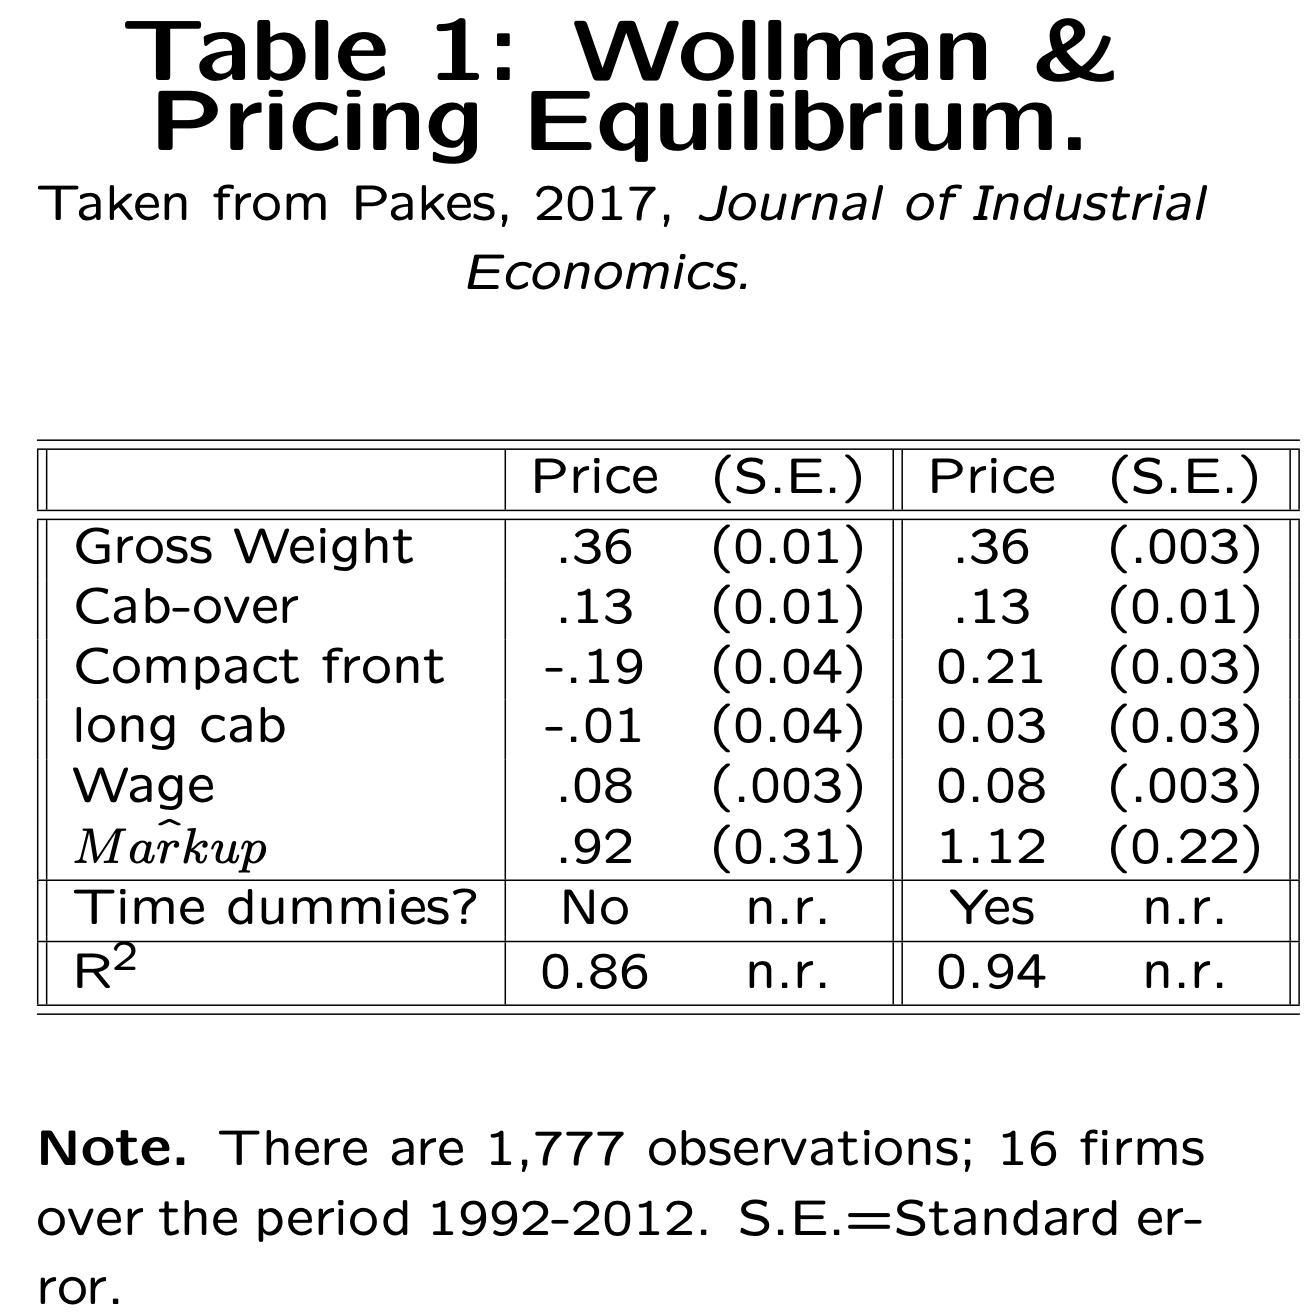
\includegraphics[height=0.9\textheight]{./resources/wollman_regression.png}
\end{center}
\end{frame}

\begin{frame}{Single Model Regressions}
These are somewhat reassuring:
\begin{itemize}
\item $\lambda\approx 1$ for multiproduct-oligopoly
\item Fit is pretty good $R^2 > 0.8$ and $R^2 > 0.5$ for within vehicle regressions (not shown).
\item As a behavioral model, multiproduct demand estimation seems successful.
\item But, do we know that an alternative $\mathcal{H}(\kappa)$ would have a $\lambda \neq 1$ or a lower $R^2$, and if so how low before we can ``reject'' the model?
\end{itemize}
\end{frame}

\begin{frame}{Goodness of Fit Tests}
Another idea (Bonnet and Dubois, Rand 2010) runs the following regression:
\begin{align*}
\log \left( p_{jt} - \eta_{jt}(\mathbf{p},\mathbf{s},\widehat{\theta}_2,\kappa) \right) &= h_s(x_{jt}, \alert{w_{jt}},\theta_3) + \omega_{jt}
\end{align*}
\begin{itemize}
\item Run a regression for each $\kappa$ and obtain $Q(\kappa)=\sum_{jt} \widehat{\omega}_{jt}^2$
\item Employ the \alert{non nested test} of Rivers and Vuong (2002). Why?
\item Working out the distribution of $Q(\kappa_1) - Q(\kappa_2)=T(\kappa_1,\kappa_2)$ is the hard part.
\item Also this is OLS (or NLLS) and there are no instruments or \alert{exclusion restrictions} for the supply side. Presumably we could add some and do GMM? (I think this is the ``formal'' test of Villas Boas (ReStud 2007)).
\end{itemize}
\end{frame}


\begin{frame}{Villas Boas (2007)}

\begin{columns}
\begin{column}{0.5\textwidth}
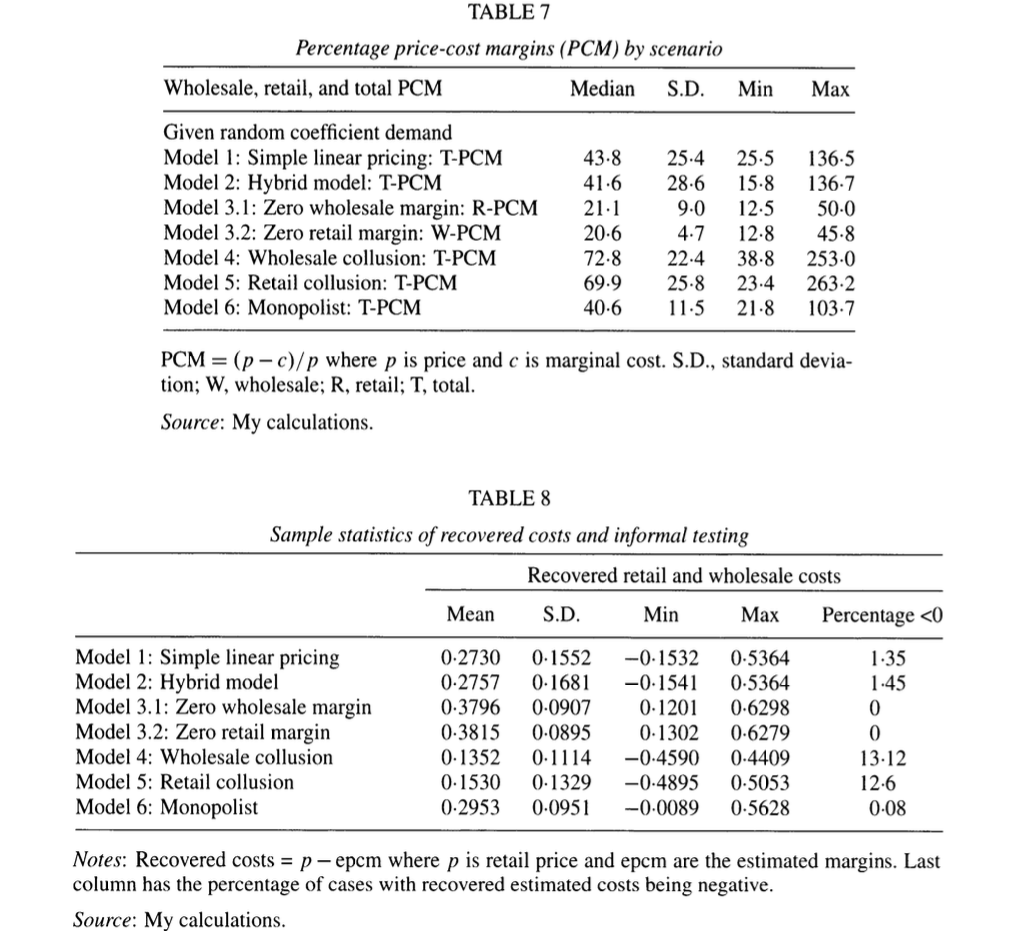
\includegraphics[height=0.9\textheight]{resources/villas_boas_table8.png}
\end{column}
\begin{column}{0.5\textwidth}
\begin{itemize}
\item Try out different models of price setting behavior, compute $\eta$ markups.
\item Unsurprisingly models with higher markups also have more costs $MC < 0$.
\item Is this evidence of incorrect conduct assumption or inelastic demand?
\end{itemize}
\end{column}
\end{columns}
\end{frame}

\begin{frame}{Villas Boas (2007)}
\begin{columns}
\begin{column}{0.6\textwidth}
\begin{center}
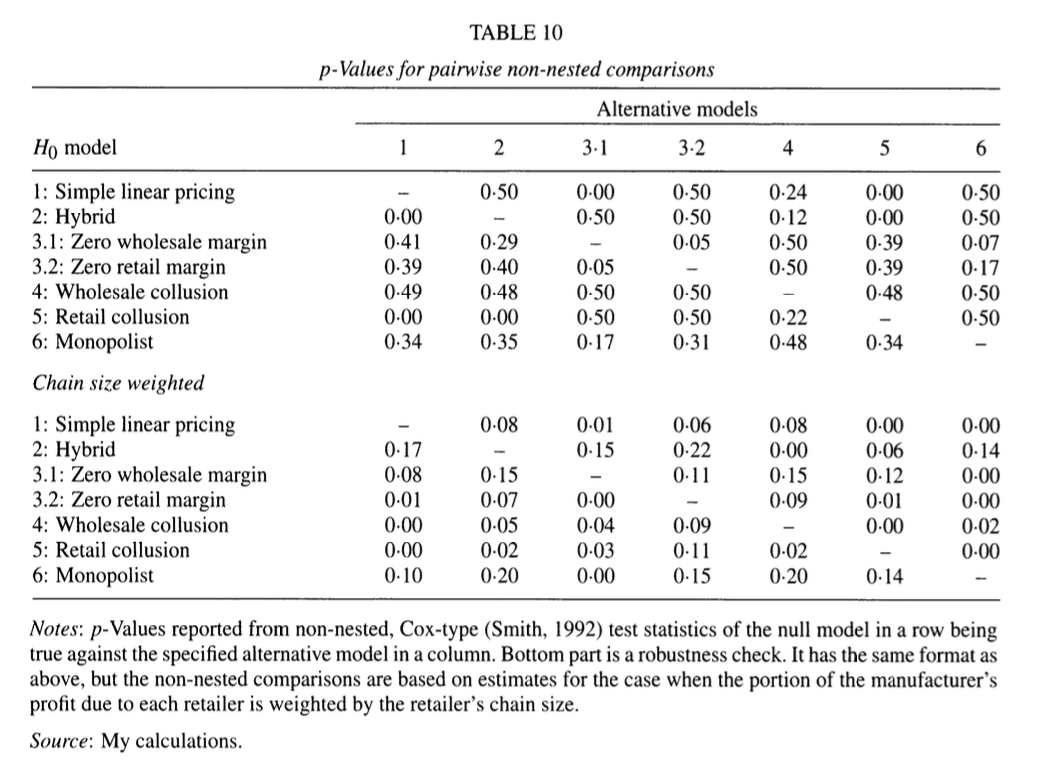
\includegraphics[height=0.9\textheight]{resources/villas_boas_table10.png}
\end{center}
\end{column}
\begin{column}{0.4\textwidth}
\begin{itemize}
\item Cox test has pairwise rejection problem (4) rejects (5) and (5) rejects (4).
\item Likewise for 3.1 and 3.2 in top panel.
\end{itemize}
\end{column}
\end{columns}


\end{frame}



\begin{frame}{Recap}
\small
So far three approaches to exploit $ E[\omega_{jt} | x_{t},w_{t},z_{t}]=0$
\begin{enumerate}
\item Put the markup on RHS and instrument for it to test $\lambda=1$ (Wald)
\begin{align*}
 p_{jt} &= h_s(x_{jt}, \alert{w_{jt}},\theta_3) + \lambda \cdot \eta_{jt}\left(\mathbf{p},\mathbf{s},\widehat{\theta_2},\kappa \right)+  \omega_{jt}
\end{align*}
\item Put the markup on LHS assuming $\lambda=1$ and test goodness of fit of supply equation (Anderson Rubin)
\begin{align*}
 p_{jt} -\eta_{jt}\left(\mathbf{p},\mathbf{s},\widehat{\theta_2},\kappa \right)&= h_s(x_{jt}, \alert{w_{jt}},\theta_3) +  \omega_{jt}
\end{align*}
\item Estimate supply and demand simultaneously $[\theta_1,\theta_2,\theta_3]$ and compare goodness of fit for different $\kappa$. (Likelihood Ratio)
\end{enumerate}

\end{frame}

% \begin{frame}{Simultaneous Problem: Menu Approach}
% Assume two models of conduct (correct: $\kappa_0$) (incorrect: $\kappa_1$)
% \begin{align*}
% %\label{eq:both_mc}
% f(p_{jt} -\eta_{jt}(\kappa_0))= h(\textrm{x}_{jt},\textrm{w}_{jt};\theta_3^0)+\omega_{jt}^{0},\\
% f(p_{jt} -\eta_{jt}(\kappa_1))= h(\textrm{x}_{jt},\textrm{w}_{jt};\theta_3^1)+\omega_{jt}^{1}.
% \end{align*}
% Write things in terms of the markup difference:
% \begin{align*}
% p_{jt} -\eta_{jt}(\kappa_1)= h(x_{jt},w_{jt};\theta_3)+ \overbrace{\lambda \cdot  \Delta \eta_{jt}(\mathbf{p},\mathbf{s},\theta,\kappa_0,\kappa_1) +   \omega_{jt}}^{\widetilde{\omega_{jt}}}
% \end{align*}
% Tempting idea: run the above regression and test if $\lambda=0$.
% \begin{itemize}
% \item True model $\lambda=0$, alternate model $\lambda \neq 0$.
% \item True model will satisfy $E[\widetilde{\omega}_{jt} | x_{t}, \alert{w_{t}}, \alert{v_{t}}]=0$
% \item $\eta_{jt}$ is \alert{endogenous}: it depends on everything including $(\xi,\omega)$.
% \end{itemize}
% \end{frame}


% \begin{frame}{A subtle solution}
% \begin{itemize}
% \item Berry Haile 2014 tell us we need \alert{marginal revenue shifters} to act as \alert{exclusion restrictions}.
% \item Needs to be uncorrelated with $p_{jt}-\eta_{jt}(\kappa_0)$ but correlated with $p_{jt}-\eta_{jt}(\kappa_1)$
% \begin{itemize}
% \item If my marginal cost is correlated with marginal costs of other products or ``closeness of competitors'', I've got the wrong conduct assumption!
% \end{itemize}
% \item We need an instrument for $\Delta \eta_{jt}(\mathbf{p},\mathbf{s},\theta,\kappa_0,\kappa_1)$
% \begin{itemize}
% \item Maybe not so hard since it is basically a function of everything.
% \item Cannot have a direct effect on $mc_{jt}$ (exclusion restriction).
% \end{itemize}
% \end{itemize}
% \end{frame}



% \begin{frame}{Backus, Conlon, Sinkinson (2020)}
% What would a really good instrument look like?
% \begin{itemize}
% \item Chamberlain (1987) style optimal IV for $\kappa_{fg}$ would be $E\left[\frac{\partial \eta_{jt}(\theta_2,\mathbf{s},\mathbf{p},\kappa)}{\partial \kappa_{fg}} | x_{t}, w_{t}, v_{t}\right]$
% \begin{itemize}
% \item But infeasible without knowledge of $(\kappa,\xi,\omega)$!
% \item We could try to recover the infeasible estimate and project it onto $(x_t,w_t,v_t)$ (note: lack of $j$ subscripts!)
% \end{itemize}
% \item Menu approach: could look at discrete analogue: $E\left[\Delta \eta_{jt}(\kappa_1,\kappa_0,\theta_2,\mathbf{s},\mathbf{p}) | x_{t}, w_{t}, v_{t}\right]$
% \begin{itemize}
% \item I would need to know $\kappa_1,\kappa_0$.
% \item Still infeasible but could run a first-stage regression
% \end{itemize}
% \end{itemize}
% \end{frame}



% \begin{frame}{Backus, Conlon, Sinkinson (2020)}
% What would a really good instrument look like?
% \begin{itemize}
% \item Chamberlain (1987) style optimal IV for $\kappa_{fg}$ would be $E\left[\frac{\partial \eta_{jt}(\theta_2,\mathbf{s},\mathbf{p},\kappa)}{\partial \kappa_{fg}} | x_{t}, w_{t}, v_{t}\right]$
% \begin{itemize}
% \item But infeasible without knowledge of $(\kappa,\xi,\omega)$ so we take expectation over exogenous variables.
% \item We could try to recover the infeasible estimate and project it onto $(x_t,w_t,v_t)$ (note: lack of $j$ subscripts!)
% \end{itemize}
% \item Menu approach: could look at discrete analogue: $E\left[\Delta \eta_{jt}(\kappa_1,\kappa_0,\theta_2,\mathbf{s},\mathbf{p}) | x_{t}, w_{t}, v_{t}\right]$
% \begin{itemize}
% \item I would need to know $\kappa_1,\kappa_0$.
% \item Still infeasible but could run a first-stage regression
% \end{itemize}
% \end{itemize}
% \end{frame}


% \begin{frame}{Backus, Conlon, Sinkinson (2020)}
% \footnotesize
% Our procedure ((1)+(2) can be done separately)
% \begin{enumerate}
% \item Run OLS to obtain $\widehat{\omega}_1,\widehat{\omega}_2$ for $(\kappa_1,\kappa_2)$
% \begin{align*}
% \log \left( p_{jt} - \eta_{jt}(\mathbf{p},\mathbf{s},\widehat{\theta}_2,\kappa) \right) = h_s(x_{jt}, w_{jt},\theta_3) + \omega_{jt}
% \end{align*}
% \item Recover $\Delta \widehat{\eta}_{jt}(\kappa_1,\kappa_2)$ via nonparametric regression/machine-learning
% \begin{align*}
% \Delta \widehat{\eta_{jt}}(\kappa_1,\kappa_2) = E \left[\Delta \eta_{jt}(\kappa_1,\kappa_2) | z_{t},w_{t},x_{t} \right]
% \end{align*}
% \item Compute the violations of the moment condition
% $Q\left(\kappa^{m}\right)=\left(n^{-1} \sum_{j, t} \hat{\omega}_{j t}^{m} \cdot \widehat{\Delta \eta}_{j t}\right)^{2}$
% \item Compute the test statistic: $T=\frac{\sqrt{n}\left(Q\left(\kappa^{1}\right)-Q\left(\kappa^{2}\right)\right)}{\hat{\sigma}}$ and bootstrap the standard error.
% \end{enumerate}
% Techincally we should \alert{sample split} and estimate the the regressions on \alert{independent} samples.
% \end{frame}


% \begin{frame}{Backus, Conlon, Sinkinson (2020) [Alternative]}
% \begin{align*}
%  p_{jt} -\eta_{jt}\left(\mathbf{p},\mathbf{s},\widehat{\theta_2},\kappa \right)&= h_s(x_{jt}, \alert{w_{jt}},\theta_3) +  \omega_{jt}
% \end{align*}
% \begin{itemize}
% \item We can also directly test violations of $E[\omega_{jt} | x_t, v_t, w_t]$ by comparing resulting CUE or GEL (or GMM) objective values.
% \item Probably want to include approximate optimal IV $E\left[\frac{\partial \eta_{jt}(\theta_2,\mathbf{s},\mathbf{p},\kappa)}{\partial \kappa_{fg}} | x_{t}, w_{t}, v_{t}\right]$ in instrument set.
% \end{itemize}
% \end{frame}









\section{Backus Conlon Sinkinson (2022)}




\begin{frame}{Basic Setup}
We start with marginal revenue and marginal cost (unobserved $\omega$, observed $h(\cdot)$)
\begin{align*}
\psi_{jt}^{m} &= mc_{jt} \\
p_{jt} -\eta_{jt}^m &= h_s(\textrm{x}_{jt},\textrm{w}_{jt})  + \omega_{jt}^m
\end{align*}
\begin{itemize}
\item Let's be vague/flexible with $h_s(\cdot)$ for now, but I don't know the production function.
\item Assume: Demand and hence $\eta_{jt}^{m}$ are \alert{known (given conduct)}.\\
\item Idea $(\eta^{A},\eta^{B})$ are monopoly/perfect competition or Cournot/Bertrand.
\end{itemize}
\end{frame}



\begin{frame}{Setup: Challenges}
The true model for markups (conduct) will satisfy the CMR: $\mathbb{E}[\omega_{jt} | z_{jt}^s]=0$
\begin{align*}p_{jt} - \eta_{jt}^{(m)} &= h_s(\textrm{x}_{jt}, \textrm{w}_{jt}; \theta_3) + \omega_{jt}
\end{align*}
Goal is test two competing markups $\eta_{jt}^{(A)},\eta_{jt}^{(B)}$, but there are challenges:

\begin{enumerate}
\item Test will depend on how we choose \alert{unconditional moment restrictions} $\mathbb{E}[\omega_{jt} \cdot \, A(z_{jt}^s)]=0$

\item Test may depend on how we specify $h_s(\cdot)$
\begin{itemize}
\item All tests are basically joint tests of the specification for \alert{observed marginal costs} and the  \alert{exclusion restriction}.
\item Villas Boas (2007) tries log, linear, exponential in $x \beta $
\end{itemize}

\item Choice of $\eta_{jt}^{(m)}$ will affect our choice of \alert{weighting matrix} and thus the test. (Hall Pelletier (2011))
\end{enumerate}
\end{frame}




\begin{frame}{The Question}
Two competing markups $(\eta_{jt}^A, \eta_{jt}^B)$: which fits the data better?\\
(both may be misspecified)
\begin{align*}
p_{jt} = h_s(\textrm{x}_{jt},\textrm{w}_{jt}) + \tau\, \eta_{jt}^A + (1-\tau)\,\eta_{jt}^B + \omega_{jt}
\end{align*}
Model is defined by a conditional moment restriction $\mathbb{E}[\omega_{jt}  | z_{jt}^s]=0$
\begin{itemize}
\item $H_0: \tau =1 \text{ vs } H_a: \tau = 0$
\item This is a \alert{model selection} problem or a \alert{non nested testing} problem.
\begin{itemize}
\item We might want to compare more than two alternatives (too bad).
\end{itemize}
\item Obvious endogeneity problem with $\eta_{jt}$!
\end{itemize}
\end{frame}



\begin{frame}{Our Idea \#1: Optimal IV (again)}
Given the CMR $\mathbb{E}[\omega_{jt}  | z_{jt}^s]=0$ we can ask what is the optimal IV for moment $\mathbb{E}[\omega_{jt}' A(z_{jt}^s)]=0$:\\
\vspace{0.25cm}
Solve for $\omega_{jt}$
\begin{align*}
\omega_{jt} &= p_{jt} - h_s(\textrm{x}_{jt},\textrm{w}_{jt}) + \tau\, \eta_{jt}^A + (1-\tau)\,\eta_{jt}^B
\end{align*}
\begin{itemize}
  \item What is $\frac{\partial \omega_{jt}}{\partial \tau}?: \quad A(z_t) = \E[\eta_{jt}^A - \eta_{jt}^B \mid \mathbf{x_t}, \mathbf{w_t}, \mathbf{v_t}, \textrm{y}_t]$
  \item This looks like a \alert{first stage} (nonparametric) regression of markup difference on instruments/all exogenous variables. (Newey 1990).
  \item Instruments are supposed to explain \alert{differences in endogenous markups}. 
\end{itemize}
\end{frame}


\begin{frame}[plain,label=misspecification]{Our Idea: Motivation \#2 (Misspecification)}
Index the \alert{true} model by $0$. Then,
$$ p_{jt} -\eta^0_{jt}= h_s(x_{jt},w_{jt}) + \omega^0_{jt}.$$
To motivate a useful test, we ask what happens when we estimate supply with the \alert{wrong} conduct model (1):

$$p_{jt} -\eta_{jt}^1 = h_s(x_{jt},w_{jt}) + \underbrace{\underbrace{\eta^0_{jt} - \eta^1_{jt}}_{\equiv \Delta \eta_{jt}^{0,1}} +  \omega_{jt}^{0}}_{\omega_{jt}^{1}}.$$
\begin{itemize}
\item Misspecifying conduct introduces an omitted variable: the difference in markups.
\item Our test is premised on detection of this omitted variable.
\end{itemize}
% \hyperlink{advantages}{\beamerskipbutton{back}} 
\end{frame}


\begin{frame}[plain,label=innovation]{Our Innovation: How does this help?}
\begin{small}
The model is given by
$$p_{jt} - \eta^m_{jt} = h_s(\cdot) +  \omega^m_{jt} \text{,   and  } \mathbb{E}[\omega_{jt}^{(m)}\cdot A(z_t)] = 0.$$

We suggest $A(z_t) = \mathbb{E}[\eta^1_{jt}-\eta_{jt}^2|z_{t}]$; several advantages:

\begin{itemize}
% \item What is the point of instruments for testing? To explain the \alert{difference in markups}
\item Reduces potentially many moments ($\mathbb{E}[\omega_{jt}' z_t]=0$) to a single, scalar moment. No need for a weighting matrix, or associated problems.
\item Testing is reduced to two prediction exercises: $\mathbb{E}[\eta^1_{jt}-\eta_{jt}^2|z_{t}]$ and $\widehat \omega_{jt}^{(m)}$.
\item Show in the paper that this leads to the most powerful test (maximizes distance between two GMM objective functions conditional on weight matrix).
\item Downside: Our choice of instrument is \alert{model specific}! UMP is not going to happen.
\end{itemize}
\end{small}
\end{frame}



\begin{frame}{Testing Environment}
Compare violations of unconditional moments under $(\eta_{jt}^A, \eta_{jt}^B)$ and $A(z_{jt}^s)$:
\begin{align*}
p_{jt} -  \eta_{jt}^A = h_s(\textrm{x}_{jt},\textrm{w}_{jt}) + \omega_{jt}^{A}\\
p_{jt} -  \eta_{jt}^B = h_s(\textrm{x}_{jt},\textrm{w}_{jt}) + \omega_{jt}^{B}
\end{align*}
These are just \alert{nonparametric regressions}.\\

Which gives us
\begin{align*}
g_A = \frac{1}{N} \sum_{jt} \omega_{jt}^{A}\, A(z_{jt}^s), &\quad
g_B =\frac{1}{N} \sum_{jt}  \omega_{jt}^{B}\, A(z_{jt}^s)\\
Q_m &= g_m'\, W_m\, g_m
\end{align*}
Now consider a \alert{Rivers Vuong (2002)} type test $T_{RV} = \sqrt{n} \left(\frac{Q_A - Q_B}{\sigma_{Q_A - Q_B}}\right) \sim N(0,1)$
$H_0: Q_A - Q_B=0$ vs. $H_A: Q_A > Q_B$ or $Q_A < Q_B$.\\
Getting the SD of the difference is hard $\rightarrow$ bootstrap 
\end{frame}



\begin{frame}[shrink=25,plain]{Algorithm}
\begin{enumerate}[(1)]
\item Split the sample by markets $t$ into 70\% \textit{test} and 30\% \textit{train}.
\item On the \textit{training sample}:
\begin{enumerate}[(a)]
\item Approximate the optimal instruments $a(z_{jt}^s) = \mathbb{E}[\Delta \eta_{jt}^{(1,2)} \mid z_{jt}^s]$ as the fitted values from:
\begin{align*}
    \Delta\eta_{jt}^{1,2} = g(z_{jt}^s) + \zeta_{jt}.
\end{align*}
\item Estimate the marginal cost function, under models 1 and 2 to obtain residuals $\widehat{\omega_{jt}^{1}}$ and $\widehat{\omega_{jt}^{2}}$:
 \begin{align*}
 p_{jt} -\eta^m_{jt}= h_s(\textrm{x}_{jt},\mathrm{w}_{jt}; \theta_3) + \omega^m_{jt}.
 \end{align*}
\end{enumerate}
\item On the \textit{test sample}:
\begin{enumerate}[(a)]
\item For each candidate model, compute the value of the scalar moment:\footnotemark
\begin{align*}
 Q(\eta^m) =\left(\sum_{j,t} \hat\omega_{jt}^m\cdot \hat{g}(\mathbf{z_t}) \right)^2.
\end{align*}
\item Repeat the previous step on bootstrapped samples and estimate $\hat\sigma/\sqrt{n}$ the standard error of the difference $\tilde Q(\eta^1) - \tilde Q(\eta^2)$.
\item Compute the test statistic
\begin{align*}
T = \frac{\sqrt{n} \left(Q(\eta^1) -  Q(\eta^2) \right)}{\widehat{\sigma}} \sim \mathcal{N}(0,1).
\end{align*}
\textit{Note: Steps 2(a) and 2(b) can be done in any order via non-parametric regression.}
\end{enumerate}
\end{enumerate}
\end{frame}





\begin{frame}{Comparison to Literature}
\begin{itemize}
\item Bresnahan (1987): Did LR test to determine collusion vs. competition in 1955 automobile price war
\begin{itemize}
\item No IV, errors were measurement in $P,Q$.
\end{itemize}
\item Bonnet and Dubois (2010): RV test
\begin{itemize}
\item But no IV -- maximum likelihood with normally distirbuted $\omega_{jt}$'s.
\end{itemize}
\item Villas Boas (2007): Cox test to determine double marginalization or not in yogurt
\begin{itemize}
\item GMM objective, unclear what if any IV are used.
\item Need to ``know'' the true model.
\end{itemize}
\item Duarte, Magnolfi, Solvsten, Sullivan (2022): RV beats Cox pretty badly in Monte Carlo.
\end{itemize}
\end{frame}



\begin{frame}[plain]{Limitations}
Not everything is testable:
\begin{itemize}
\item If $\Delta \eta_{jt}$ cannot be explained by $z_{jt}^s$ beyond contents of $(\mathrm{x}_j,\mathrm{w}_j)$ we have nothing
%\item Compare perfect competition to a fixed markup $p_j = a \cdot mc_j + b$
\item Flexible demand models are required to generate cross sectional variation in markups
%\begin{itemize}
\item Discuss plain logit
%\end{itemize}
\item Beware of ``accidental'' exclusion restrictions.
\end{itemize}
\end{frame}


\section{Examples}


\begin{frame}{Scuderi JMP 2022: Models of Labor Supply}
\begin{columns}
\begin{column}{0.7\textwidth}
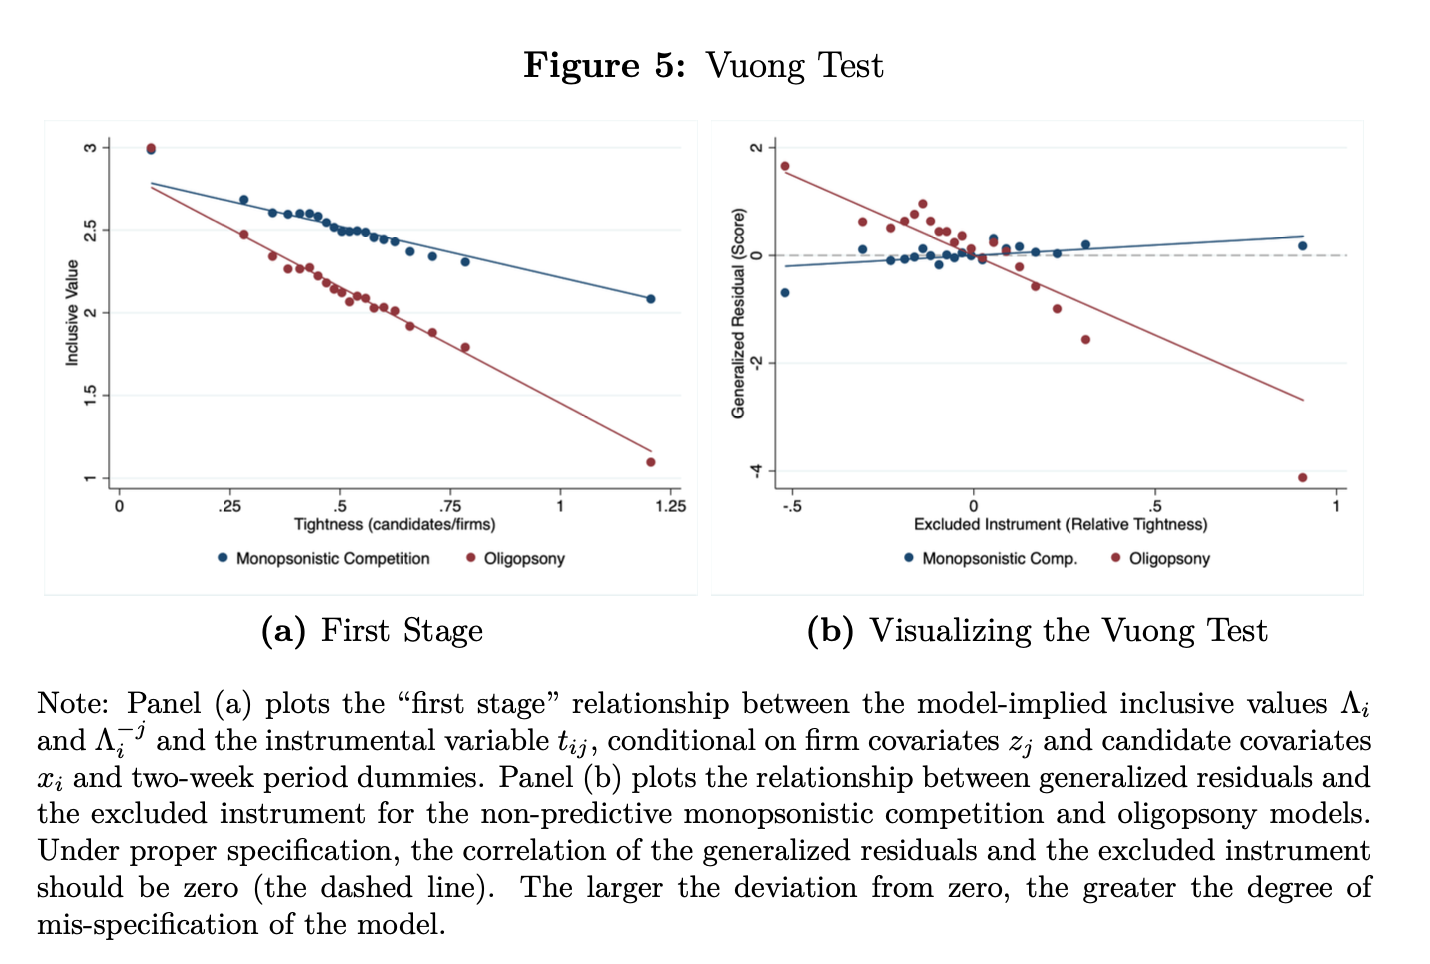
\includegraphics[height=0.9\textheight]{resources/scuderi1}
\end{column}
\begin{column}{0.3\textwidth}
\begin{itemize}
\item Offered wages for online job platform
\item Compares Monopsony vs. oligopolistic competition vs. perfect comp.
\item Compares tailored offers vs. not (price discrimination).
\end{itemize}
\end{column}
\end{columns}
\end{frame}


\begin{frame}{Scuderi JMP 2022: Models of Labor Supply}
\begin{columns}
\begin{column}{0.5\textwidth}
\begin{itemize}
\item Firms ignore competitors (Monopsony)
\item Firms offer wages independent of candidate characteristics (experience, demographics).
\item Firms are definitely NOT paying MPL.
\end{itemize}
\end{column}
\begin{column}{0.5\textwidth}
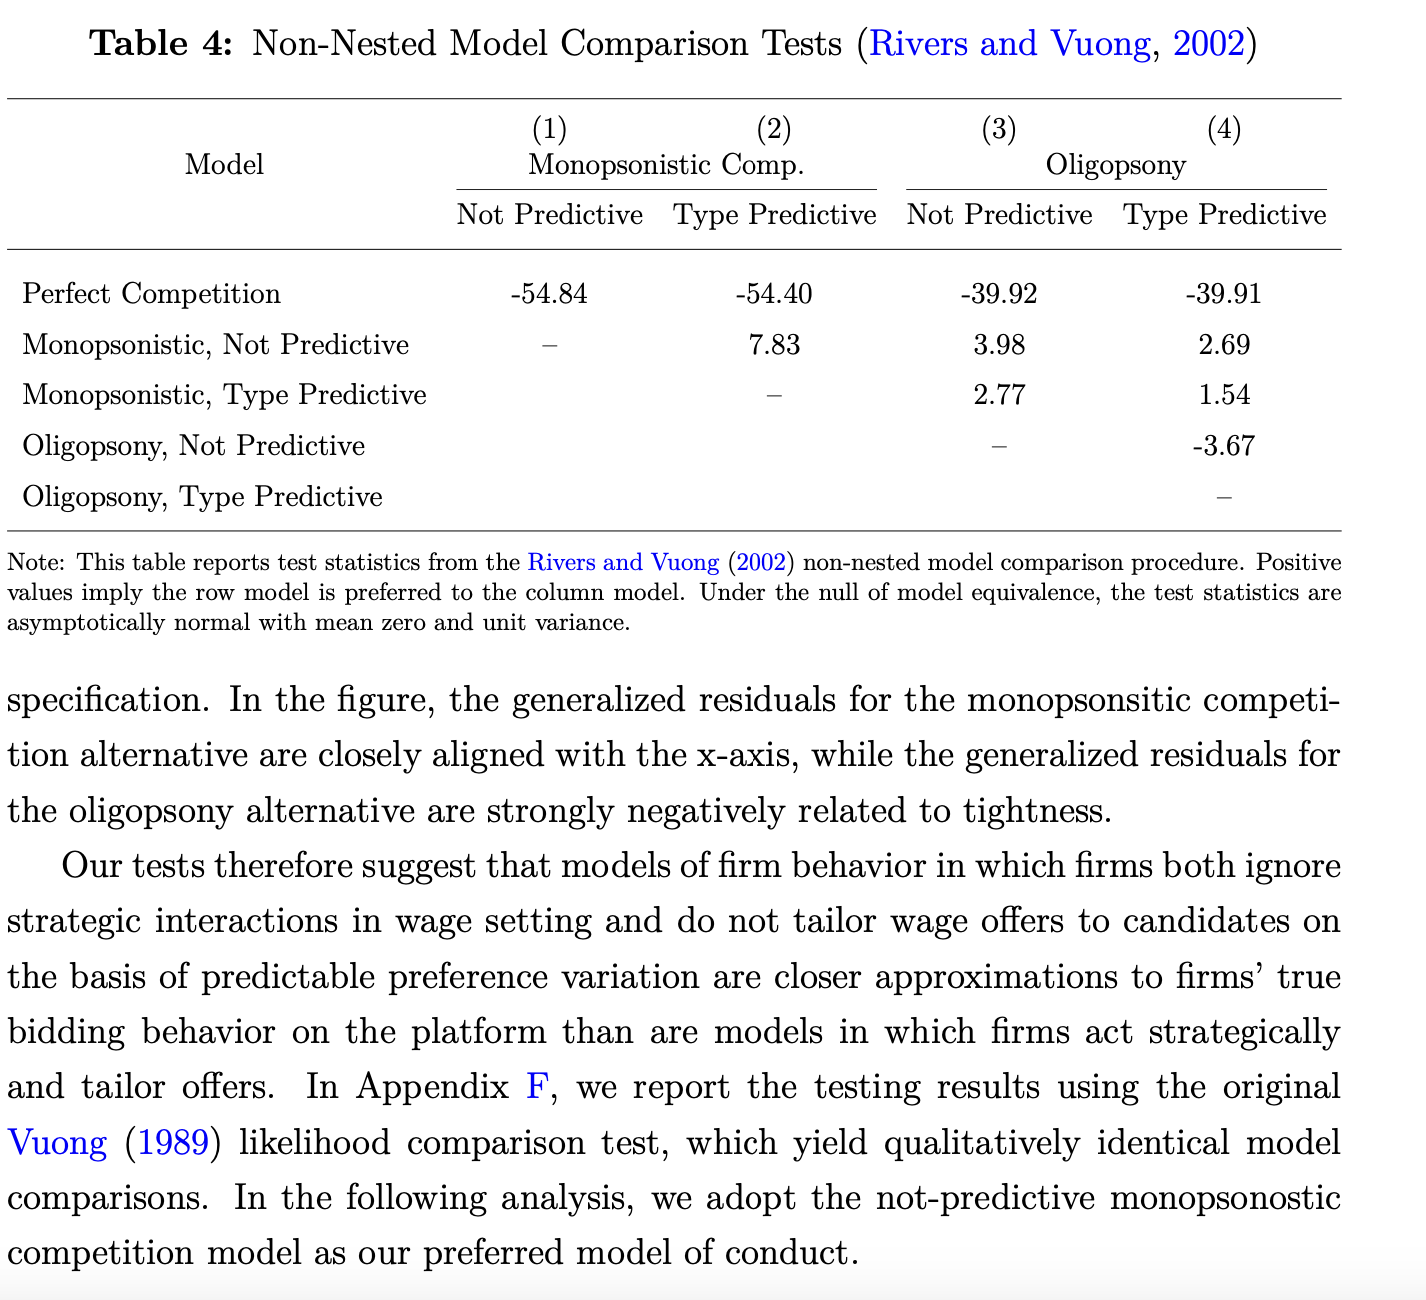
\includegraphics[height=0.9\textheight]{resources/scuderi2}
\end{column}
\end{columns}
\end{frame}

\begin{frame}{Starc Wollmann: Generic Pharma Cartel + Entry}
Do Cartels encourage entry with high prices?\\
\vspace{0.25cm}
\begin{quote}
in 2013, Teva Pharmaceuticals, the largest generic firm, hired NP, a marketing executive with especially strong industry relationships, and tasked her with "price increase implementation."1 Over an 18-month period, industry participants exchanged thousands of calls and texts—alongside countless LinkedIn, Facebook, and WhatsApp messages and face-to-face conversations—with contacts at rival firms to coordinate the increases (Complaint, page 322).2 Following this period, prescription drug expenditures by governments, private insurers, and individuals rose sharply by billions of dollars.
\end{quote}
\end{frame}



\begin{frame}{Starc Wollmann: Generic Pharma Cartel }
\begin{columns}
\begin{column}{0.5\textwidth}
\begin{itemize}
\item NP organizes the cartel and prices go up
\item Slightly less in large markets (which are more likely to see entry)
\end{itemize}
\end{column}
\begin{column}{0.5\textwidth}
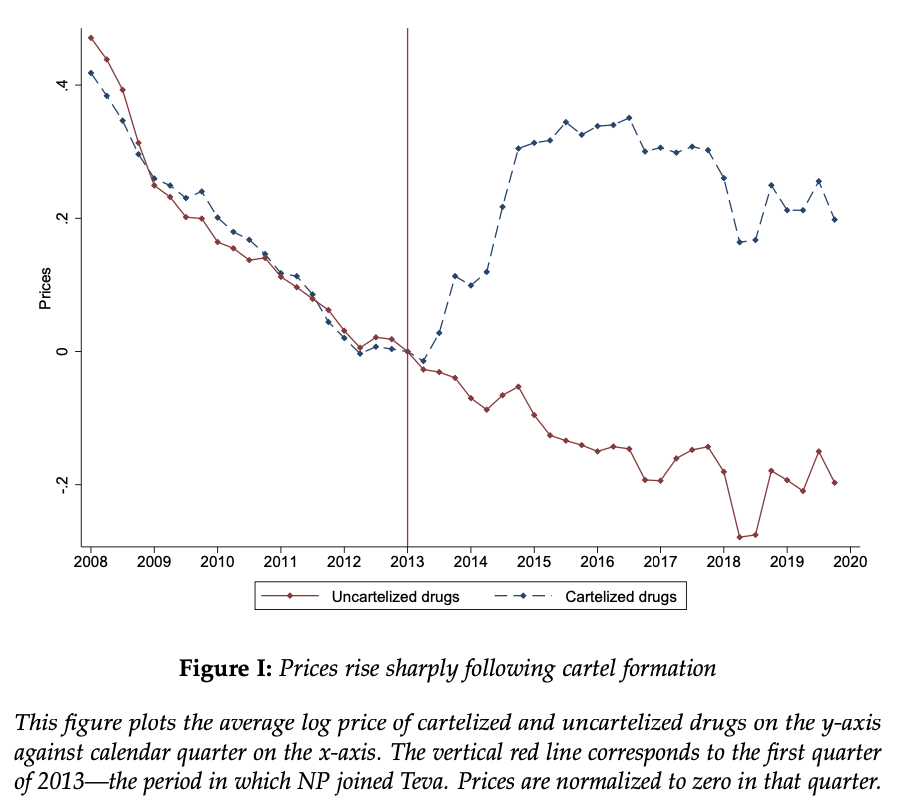
\includegraphics[height=0.85\textheight]{resources/starc_1}
\end{column}
\end{columns}
\end{frame}


\begin{frame}{Star Wollmann: Baseline Scenario }
\begin{itemize}
\item all firms set competitive prices in uncartelized markets
\item all firms set competitive prices in cartelized markets before cartel formation;
\item  and after cartel formation, members set prices that maximize their joint profits while nonmembers best respond
\end{itemize}
\end{frame}

\begin{frame}{Starc Wollmann: Testing Results }
\begin{center}
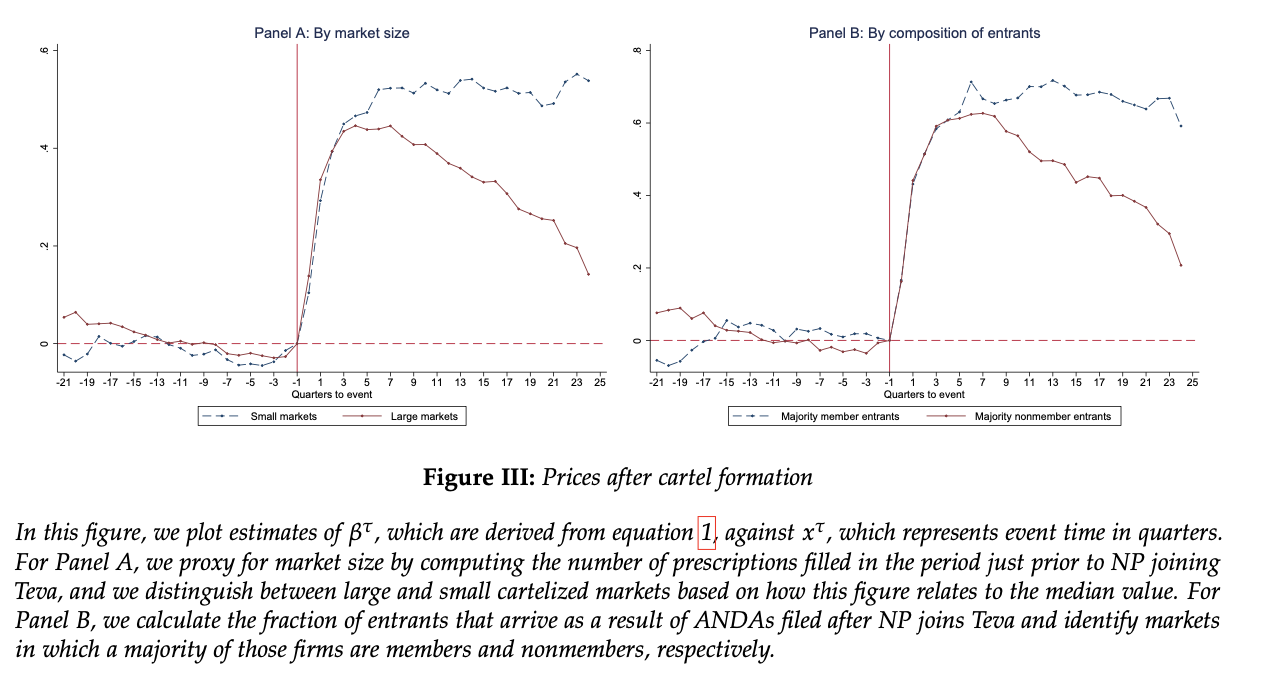
\includegraphics[height=0.85\textheight]{resources/starc_2}
\end{center}
\end{frame}

\begin{frame}{Starc Wollmann: Generic Pharma Cartel }
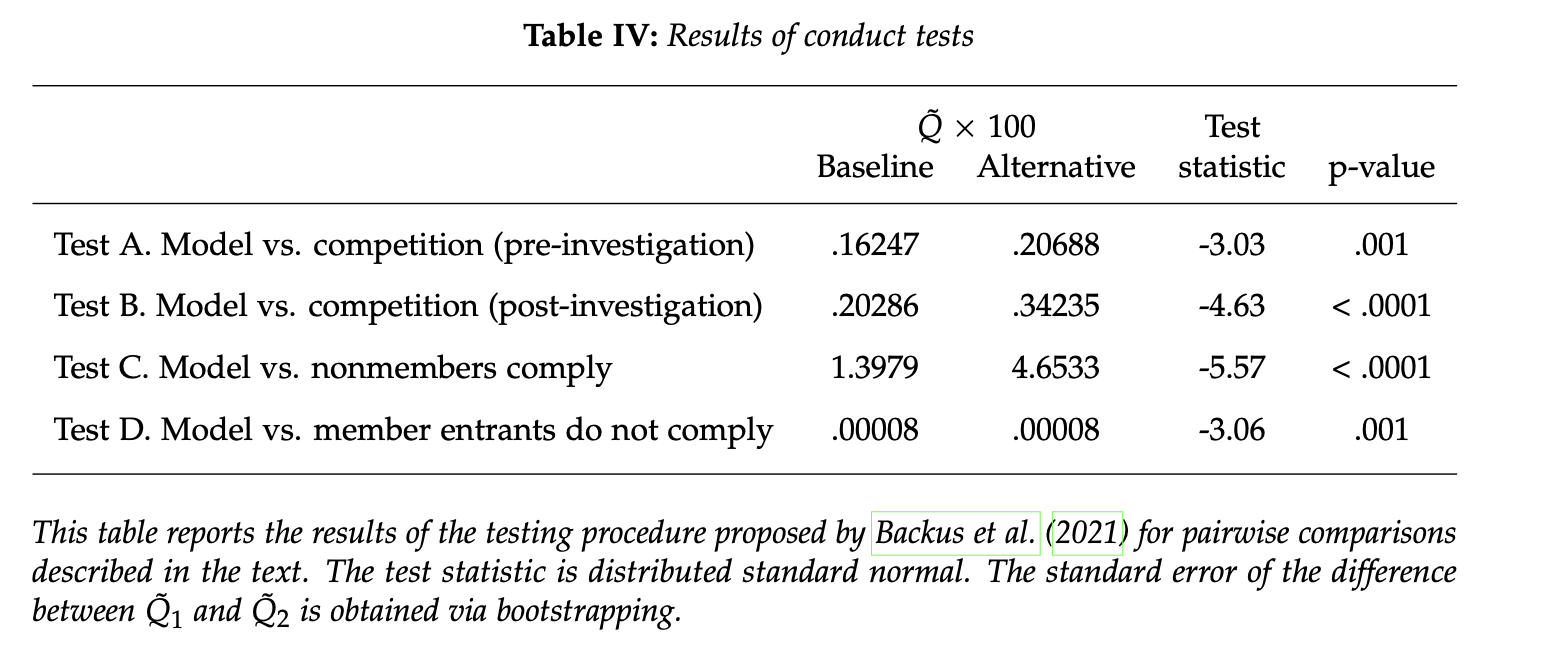
\includegraphics[height=0.85\textheight]{resources/starc_3}
\end{frame}



\begin{frame}[plain,label=mainresults]{Main Results: These are $N(0,1)$}
\begin{center}
\scalebox{0.55}{\begin{tabularx}{500pt}{l*4             {>{\Centering}X}}\toprule
{} &  Others' Cost &  Demographics &  BLP Inst. &  Dmd. Opt. Inst. \\
\midrule \multicolumn{1}{c}{Own Profit Max vs.}&             \multicolumn{4}{c}{Panel 1: $A(\mathbf{z}_t)=\mathbf{z}_t,$ linear $h_s(\cdot)$ }\\                 \cmidrule(lr){1-1} \cmidrule(lr){2-5}
%Single Product                            &        3.0840 &        1.1230 &     0.9976 &           0.6859 \\
Common Ownership                          &       -4.3410 &       -1.1966 &     0.5047 &          -1.2552 \\
Double Marginalization                    &        2.1922 &        1.0055 &    -0.0412 &           7.0897 \\
Double Marginalization + CO &       -0.8262 &        0.6892 &     0.1428 &           6.9320 \\
Perfect Competition                       &        3.2995 &        0.5194 &     0.7355 &           3.7223 \\
Monopolist                                &       -2.2264 &       -1.0528 &    -0.4525 &          -0.9202 \\

 \midrule 

\multicolumn{1}{c}{Own Profit Max vs.}& \multicolumn{4}{c}{Panel 2:             $A(\mathbf{z}_t)=\mathbb{E}[\Delta \eta^{12}|\mathbf{z_t}]$, linear $h_s(\cdot)$ and $g(\cdot)$}\\                            \cmidrule(lr){1-1} \cmidrule(lr){2-5}
%Single Product                            &        1.4264 &        0.5795 &     0.6662 &           1.2368 \\
Common Ownership                          &       -2.3044 &       -0.5105 &    -0.0384 &          -1.6133 \\
Double Marginalization                    &        0.8644 &        0.4421 &    -0.5311 &           3.3367 \\
Double Marginalization + CO &       -0.9382 &       -0.2389 &    -0.3684 &          -0.0045 \\
Perfect Competition                       &        0.7164 &        0.6135 &    -0.1080 &          -0.3151 \\
Monopolist                                &       -0.8577 &       -0.4002 &    -0.3868 &          -1.2339 \\

 \midrule 

\multicolumn{1}{c}{Own Profit Max vs.}& \multicolumn{4}{c}{Panel 3:             $A(\mathbf{z}_t)=\mathbb{E}[\Delta \eta^{12}|\mathbf{z_t}]$, random forest $h_s(\cdot)$ and $g(\cdot)$}\\                    \cmidrule(lr){1-1} \cmidrule(lr){2-5}
%Single Product                            &        4.8400 &        5.0700 &     5.1738 &           5.4990 \\
Common Ownership                          &       -3.3777 &       -3.2509 &    -3.7130 &          -4.0256 \\
Double Marginalization                    &       -5.9699 &       -9.9547 &    -6.5789 &          -7.8269 \\
Double Marginalization + CO &       -5.9264 &       -6.1550 &    -6.5231 &          -7.4760 \\
Perfect Competition                       &       -4.0468 &       -6.1901 &    -5.1494 &          -6.3484 \\
Monopolist                                &       -3.4972 &       -4.0070 &    -3.4358 &          -3.7495 \\
\bottomrule
\end{tabularx}
}
\end{center}
\end{frame}
% \hyperlink{morepanels}{\beamerskipbutton{additional specifications}}\hyperlink{mcregs}{\beamerskipbutton{marginal cost regressions}}
%\hyperlink{step2regs}{\beamerskipbutton{step 2 regressions}} \hyperlink{pwregs}{\beamerskipbutton{Pakes-Wollmann regressions}}

\begin{frame}[plain]{An Internalization Parameter}
Let $\kappa$ represent the weight a firm places on competitors and $\tau$ the internalization of those weights.
 \begin{equation*}
 arg\max_{p_j \,:\, j \in \mathcal{J}_f} \sum_{j \in \mathcal{J}_f} (p_j - mc_j) \cdot s_j(\mathbf{p})+
 \sum_{g\neq f} \alert{\tau} \kappa_{fg} \sum_{j \in \mathcal{J}_g} (p_k - mc_k) \cdot s_k(\mathbf{p})
 \end{equation*}
Now, 
\begin{itemize}
\item $\tau = 0$ implies own-profit maximization
\item $\tau = 1$ implies common ownership pricing
\item $\tau$ in between is..? Agency?
\end{itemize}
We test $\tau \in (0.1, \ldots, 0.9)$ against own-profit maximization.
\end{frame}

\begin{frame}[plain]{Internalization Parameter Results}
\begin{center}
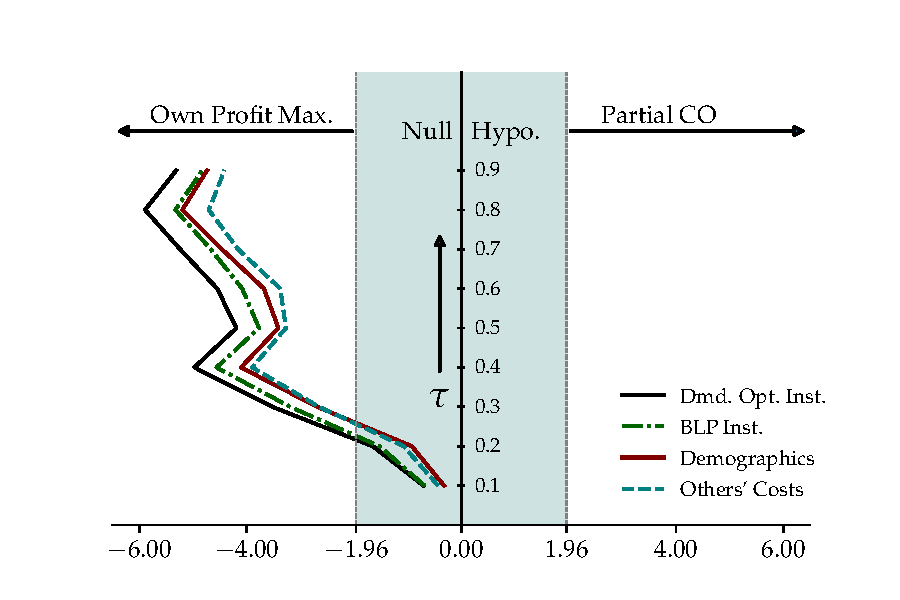
\includegraphics[width=10cm]{resources/tau_figure2.pdf}
\end{center}
\end{frame}


% \begin{frame}{Setup: Demand (BLP95, BLP99, Nevo 2000, ...)}
% Consumer $i$ makes discrete choice in market $t$ and receives utility for choice $j$:
% \begin{align*}
% u_{ijt} &=  h_d(\textrm{x}_{jt}, \textrm{v}_{jt}; \theta_1) - \alpha\, p_{jt} + \lambda \, \log(\text{ad}_{jt}) + \xi_{jt}  + \mu_{ijt}(\textrm{x}_{jt}, y_i; \widetilde{\theta}_2) + \varepsilon_{ijt}
% \end{align*}
% 
% Following Berry, Levinsohn, Pakes, we fix $\theta_2=[\widetilde \theta_2,\alpha, \lambda]$ and invert system of equations for $\mathcal{S}_t$ to get mean utilities:
% \begin{align*}
% \sigma_{j}^{-1}(\mathcal{S}_t, \chi_t, \mathbf{p_t},\mathrm{y_t}; \widetilde{\theta}_2) + \alpha\, p_{jt} - \lambda \, \log(\text{ad}_{jt}) &= h_d(\textrm{x}_{jt}, \textrm{v}_{jt}; \theta_1) + \xi_{jt} 
% \end{align*}
% Can estimate $[\widehat{\theta_1}, \widehat{\theta_2}]$ using the CMR $\mathbb{E}[\xi_{jt} | z_{jt}^d]=0$.
% \end{frame}

% \begin{frame}{Setup: Supply and Conduct}
% Assume that we know $\widehat{\theta_2}$ from demand:
% \begin{align*}
% p_{jt} - \eta_{jt}(\mathcal{S}_t, \chi_t, \mathbf{p_t},\mathrm{y_t}; \widehat{\theta}_2) = h_s(\mathrm{x}_{jt}, \mathrm{w}_{jt}, q_{jt}; \theta_3) + \omega_{jt} \quad &\text{ with } \mathbb{E}[\omega_{jt} | z_{jt}^s]=0
% \end{align*}
% \begin{itemize}
% \item The model is defined by \alert{conditional moment restrictions}.
% \item Testing conduct is typically about detecting violations of the CMR for supply.
% \item We follow the \alert{sequential approach} and estimate $[\widehat \theta_1,\widehat \theta_2]$ from demand and then test supply separately.
% \item The $\theta_3$ parameters are \alert{nuisance parameters}, we don't care what they are, we just want to measure violations of moments.
% \end{itemize}
% \end{frame}



% \begin{frame}[plain,label=chamberlain]{A Brief Aside: Chamberlain (1987) in a Slide}
% What contains as much information as the CMR $\mathbb{E}[\omega|z_{jt}^s]$ and moments of the form $ \mathbb{E}[\omega_{jt}\cdot A(z_{jt}^s)]. $
% \begin{itemize}
% \item For linear models $A(z_{jt}^s) = z_{jt}^s$ is generally without loss.
% \item For nonlinear models, Chamberlain (1987) shows that the efficient estimator uses
% $$A(z_{jt}^s) = \mathbb{E}\left[\frac{\partial \omega_{jt}}{\partial \theta}|z_{jt}^s\right]$$
% \item That is not too helpful (its a function of the unknown $\theta$).
% \item Much of the follow-up work has been about feasible approximations to this ``optimal instrument" (e.g., Newey 1990)
% \end{itemize}
% For us a similar concern arises, but it is about \alert{power} to distinguish conduct models rather than \alert{efficiency} of estimation.
% %\hyperlink{label=cmrbasics}{\beamerskipbutton{back}} 
% \end{frame}



% \begin{frame}[plain,label=innovation]{Our Idea: Motivation \#1 (Optimal IV)}
% The model is given by
% \begin{align*}
% p_{jt} &= h_s(\textrm{x}_{jt},\textrm{w}_{jt},\theta_3) + \tau \cdot \eta^A_{jt} + (1-\tau) \cdot \eta^B_{jt} + \omega^m_{jt}\\
% & \text{  where  }  H_0: \tau=1 \text{ and } H_a: \tau = 0
% \end{align*}

% \begin{itemize}
% \item The optimal IV in the Chamberlain (1987) sense is given by $\mathbb{E}\left[\frac{\partial \omega_{jt}}{\partial \tau}|z_{t} \right]= \mathbb{E}\left[\eta^A_{jt}-\eta_{jt}^B|z_{t}\right]$.
% \item In words: The IV need to predict the \alert{difference in markups}\\ (beyond observed $h_s(\textrm{x}_{jt},\textrm{w}_{jt},\theta_3)$).
% \end{itemize}
% \end{frame}








\begin{frame}{Possible Exclusion Restrictions}
We are looking for variables which affect \alert{demand but not supply}:
\begin{align*}
\sigma_{j}^{-1}(\mathcal{S}_t, \mathbf{p_t},\alert{\mathrm{y_t}}, \mathrm{x}_t,  \mathrm{v}_t, \widetilde{\theta}_2) 
&= h_d(\mathrm{x}_{jt},\alert{ \mathrm{v}_{jt}}; \theta_1) - \alpha\, p_{jt} + \lambda \, \log(\text{ad}_{jt})+ \xi_{jt} \\
p_{jt} - \eta_{jt}(\mathcal{S}_t, \mathbf{p_t}; \theta_2, \mathcal{H}_t(\kappa))
&= h_s(\textrm{x}_{jt}, \alert{\mathrm{w}_{jt}}; \theta_3) + \omega_{jt} 
\end{align*}
Things we use:
\begin{itemize}
    \item Obvious choice: $\mathrm{v}_{jt}$ (things like product recalls are relatively weak)
    \item Demographics (enter nonlinearly): $\mathrm{y}_t$ (chain-level income works well)
    \item Characteristics of other goods: $f(\mathrm{x}_{-j,t})$ (BLP instruments).
    \item Characteristics of other goods: $\mathrm{w}_{-j,t}$ (commodity price of oats for Rice Krispies)
\end{itemize}

Things we don't use:
\begin{itemize}
    \item Unobserved demand shocks $\xi_{jt}$ (see MacKay Miller 2020 for $Cov(\xi_j,\omega_j)=0$).
    \item Observable $\kappa$ conduct shifters (financial mergers/events, see Miller Weinberg (2018))
\end{itemize}
\end{frame}




\end{document}

